\documentclass[tikz,border=8pt]{standalone}
\usepackage{amsmath,amssymb}\usetikzlibrary{arrows.meta,positioning,fit}
\begin{document}
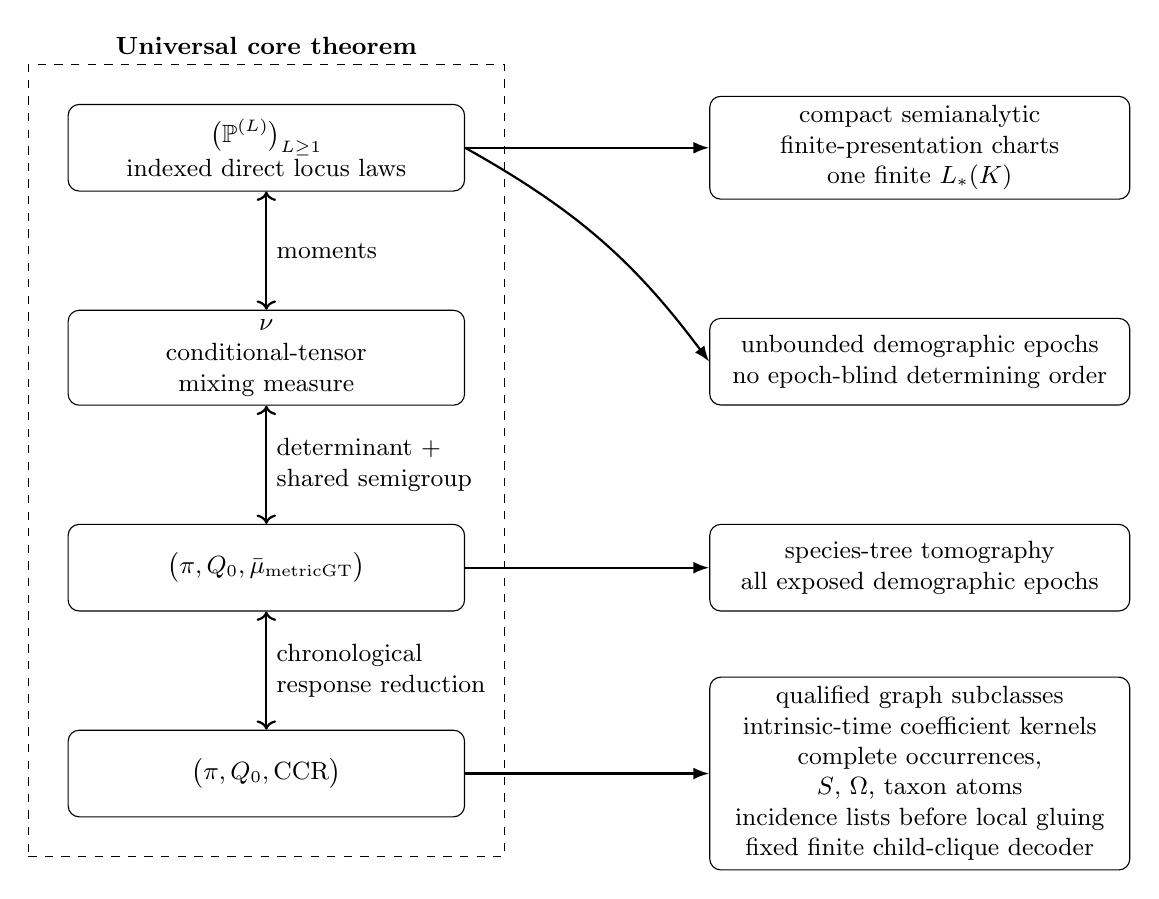
\begin{tikzpicture}[node distance=15mm and 31mm, every node/.style={font=\small}, box/.style={draw,rounded corners,align=center,text width=48mm,minimum height=11mm}, side/.style={box,text width=51mm}, arr/.style={-{Latex[length=2mm]},thick}]
\node[box] (laws) {$\bigl(\mathbb P^{(L)}\bigr)_{L\ge1}$\\indexed direct locus laws};
\node[box,below=of laws] (nu) {$\nu$\\conditional-tensor mixing measure};
\node[box,below=of nu] (triple) {$\bigl(\pi,Q_0,\bar\mu_{\rm metricGT}\bigr)$};
\node[box,below=of triple] (ccr) {$\bigl(\pi,Q_0,\operatorname{CCR}\bigr)$};
\draw[arr,<->] (laws)--node[right]{moments}(nu);
\draw[arr,<->] (nu)--node[right,align=left]{determinant +\\shared semigroup}(triple);
\draw[arr,<->] (triple)--node[right,align=left]{chronological\\response reduction}(ccr);

\node[side,right=of laws] (finite) {compact semianalytic\\finite-presentation charts\\one finite $L_*(K)$};
\node[side,below=of finite] (negative) {unbounded demographic epochs\\no epoch-blind determining order};
\node[side,right=of triple] (tree) {species-tree tomography\\all exposed demographic epochs};
\node[side,right=of ccr] (graph) {qualified graph subclasses\\intrinsic-time coefficient kernels\\complete occurrences, $S$, $\Omega$, taxon atoms\\incidence lists before local gluing\\fixed finite child-clique decoder};
\draw[arr] (laws)--(finite);
\draw[arr] (laws.east) to[bend left=12] (negative.west);
\draw[arr] (triple)--(tree);
\draw[arr] (ccr)--(graph);
\node[draw,dashed,fit=(laws)(nu)(triple)(ccr),inner sep=5mm,label=above:{\bfseries Universal core theorem}] {};
\end{tikzpicture}
\end{document}
